\documentclass{standalone}
  \usepackage{tikz}
  \usetikzlibrary{arrows, automata, positioning, shapes.misc}
  \tikzstyle{automaton}=[shorten >=1pt, >=stealth', initial text=]
  \tikzstyle{accepting}=[accepting by arrow]

\begin{document}
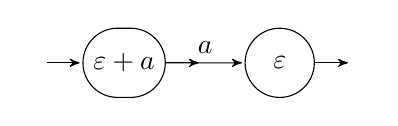
\begin{tikzpicture}[automaton, auto]
  \node[state,initial,accepting,rounded rectangle] (0) {$\varepsilon + a$};
  \node[state,accepting,rounded rectangle] (1) [right=of 0] {$\varepsilon$};
  \path[->] (0) edge node {$a$} (1);
\end{tikzpicture}
\end{document}
